% Chapter 3

\chapter{Environment} % Main chapter title

\label{Chapter3} % For referencing the chapter elsewhere, use \ref{Chapter3} 

%----------------------------------------------------------------------------------------

In this chapter we report the process that went into choosing the environments that we will be using in the project's simulations, and from which we will be basing our simulations.

There are many choices of environments and tasks that are publicly available. Some of these we will be introducing in this chapter.

What makes this step non-trivial and deserving of its own chapter is that different reinforcement learning techniques are more suitable to different categories of tasks. Similarly, different machine learning and deep learning techniques are more or less efficient when applied to different tasks.

In a research effort that is heavily dependent on building reinforcement learning and deep learning models, the choice of environment is a critical one.

Furthermore, we also need to achieve this without losing focus on the main motivations for the whole project (Chapter~\ref{Chapter1}): \textit{optimising reinforcement learning algorithms by adding transferability of pre-trained models on unseen maps or configurations of a task}.

This last point implies that a substantial part of the computational work in the project will be about training hundreds of thousands of reinforcement learning models to build a dataset over a distribution of different maps (we present this in Chapter~\ref{Chapter4}). This is an important point: in the many experiments we ran, this turned out to be the biggest bottleneck, and required plans to distribute computations across multiple machines to make the computational time feasible in the timespan allocated to the project.

With these points in mind and given the experimental nature of the work, we conclude that a bottom-up approach in complexity is preferable. Given successful results with "easier" tasks, we can scale up in complexity and hopefully formalise and generalise our approach to more tasks (Chapter~\ref{Chapter7}).

Easier tasks will enable us to explore different reinforcement learning approaches that we introduced in Subsection~\ref{RL} with the guarantee that they will give satisfiable results. We can use these results as a foundation of the further steps (specifically Generative Adversarial Networks training in Chapter~\ref{Chapter5}).

Before introducing candidate environments, let us define what is meant by an "easy" reinforcement learning task. What we are looking for is ideally a task with a discrete and relatively small set of observable states and actions. Why does this condition make the task easier?

Imagine building a decision tree (such as the one shown in figure~\ref{fig:RLTree} with all possible states-action transitions, until we either: 1) reach a goal state, or 2) reach an arbitrarily maximum iteration time step $t = \eta$ or depth of the tree (to prevent infinite iterations). Also assume we were building this tree in a bruteforce manner (worst-case scenario of reinforcement learning resolutions), such that we need to build all possible paths or trajectory that the agent will need to take. Therefore, we would need to visit each node of the tree, until we arrive at the leaves. At the leaves, we can find the achieved reward for the agent given the path it has taken to get there. 

The breath and depth of the state-action tree will increase as we increase the possible set of states we would need to traverse, adding up to the space and time complexity of our solution, which is exponential in $\#S$ and $\#A$ for both space and time ($\#S$ indicates the cardinality of a set S).

With that said, there is a solid line between our ideal environment and a trivial one that could be solved without the aid of reinforcement learning techniques.

Let's explore some candidate environments next.
\begin{figure}
\centering
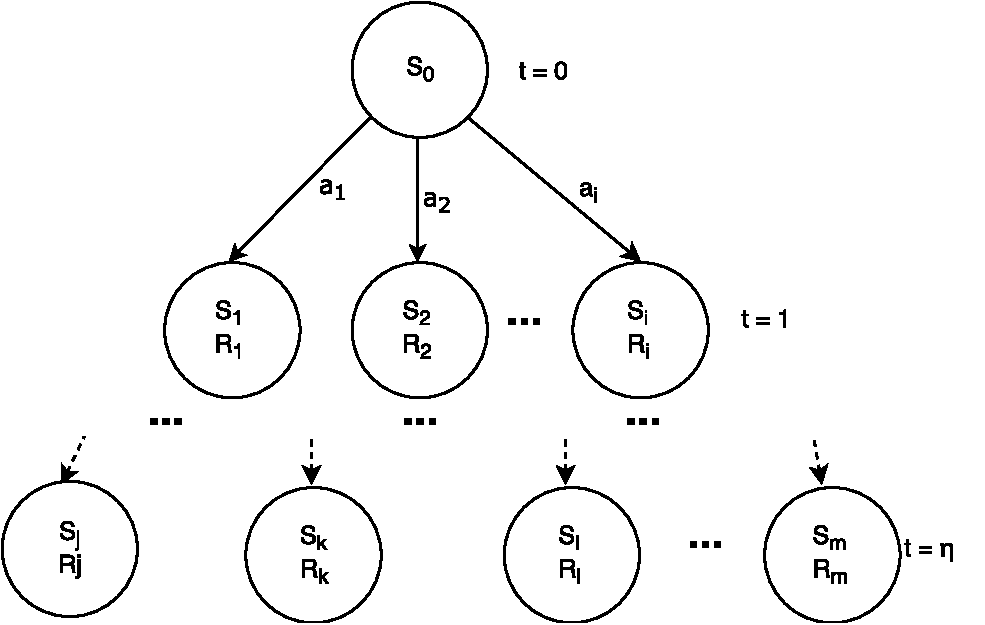
\includegraphics[width=7cm]{Figures/RLTree}
\caption{Sample state-action tree}
\label{fig:RLTree}
\end{figure}

\section{OpenAI Gym}
\label{openaigym}
OpenAI Gym \parencite{1606.01540} provides a toolkit that aids in the process of building reinforcement learning systems and evaluating algorithms to solve such tasks.

OpenAI Gym provides an environment interface \code{Env}. The interface abstracts the following operations on an environment:

\begin{itemize}
	\item \code{step(action)} -- Simulates one time step by executing the provided action. This returns \code{observation} (the new current state), the \code{reward} for taking such action, a flag \code{done} indicating whether the system has reached a final state, and \code{info} providing additional information dependent on the environment.
	\item \code{reset()} -- Resets the environment, i.e. the initial state is restored
	\item \code{render()} -- Renders the environment in human-readable format.
\end{itemize}

Now, we could either build implementations for such interface (if we were to implement our own environment's logic), or use the provided implementations for several environments in the OpenAI Gym library, which includes board games, algorithm-based or physics-based environments, Atari games, etc.

\subsection{Motivation}
In this project we will mostly deal with environments provided in the OpenAI Gym. There are several reasons for such decision:

\begin{itemize}
	\item It abstracts the need to implement the logic of a separate environment. Implementing our own environment adds a point of failure to our whole (quite experimental) work, as well as imposing a bigger time constraint to the one we already have;
	\item OpenAI Gym has become a standard academic tool for reinforcement learning researchers, therefore many papers and articles build on top of this framework;
	\item Environment implementations in the OpenAI Gym library are constantly expanding and being revised by an active community, also thanks to the support of the overarching organisation (OpenAI);
	\item The core implementation of the \code{gym} module \parencite{gymgymat12:online} allows for straightforward extensions on existing environments, which, as we will see in subsection~\ref{ExtendedBaseline}, will be critical in this project;
	\item While sadly not applicable anymore, OpenAI Gym used to provide and support an online platform for developers to compare the performance of different reinforcement learning algorithms for each task. This was in a form of a leaderboard, measuring the performances, as well as providing the implementation and data of winning techniques. Such data could have been used directly as input to our Generative Adversarial Networks.
\end{itemize}

\subsection{Algorithmic environments}
\subsection{MuJoCo and physics environments}
\subsection{Other environments}

%----------------------------------------------------------------------------------------

\section{Baseline: \code{FrozenLake-v0}}
One of our baseline environments is \code{FrozenLake-v0} \parencite{OpenAIGy42:online}, one of the algorithmic environments provided in the OpenAI Gym. In this section we describe the task, motivation for choosing it as one of our baseline models, and some shortcomings that we faced in using this environment in our project's pipeline.
\subsection{Description of the task}
In \code{FrozenLake-v0} we control an agent in a grid world, more precisely the grid shown in figure~\ref{tab:FrozenLakev0}. The objective is to go from a starting tile (\code{S}) to a goal state (\code{G}), by moving in four possible directions from a tile: \code{up}, \code{down}, \code{left} and \code{right}.

What differentiates this from a trivial path-finding or planning problem? A couple of things:
\begin{enumerate}
	\item there are both walkable and non-walkable tiles in the grid (these are respectively frozen tiles \code{F} and holes \code{H}), and
	\item tiles are "slippery", as in the agent could "slip" while navigating the grid world, meaning that the movement direction of the agent is uncertain and only partially depends on the direction we tell the agent to follow, i.e. the direction is non-deterministic.
\end{enumerate}

The reward in \code{FrozenLake-v0} is $1$ for reaching the goal state, and $0$ for being in any other state. The system stops executing when the agent falls into a hole, and the environment needs to be reset.

\begin{table}[]
\centering
\begin{tabular}{|c|c|c|c|}
\hline
\cellcolor[HTML]{68CBD0}\textbf{S} & F & F & F \\ \hline
F & \cellcolor[HTML]{CE6301}H & F & \cellcolor[HTML]{CE6301}H \\ \hline
F & F & F & \cellcolor[HTML]{CE6301}H \\ \hline
\cellcolor[HTML]{CE6301}H & F & F & \cellcolor[HTML]{32CB00}\textbf{G} \\ \hline
\end{tabular}
\caption{\code{FrozenLake-v0}'s default 4x4 configuration}
\label{tab:FrozenLakev0}
\end{table}

\subsection{Motivation and shortcomings}
\label{movationandshortcomings}
\code{FrozenLake-v0} is generally classified as a straightforward reinforcement learning task. An optimal solution could be found by creating a model of the environment, that is merely recording where frozen tiles are while exploring the grid world. This is a \emph{model-based} approach to reinforcement learning, and it is perhaps less interesting than learning by exploration, without being biased by the particular configurations of the map.

\emph{Model-free} algorithms, like Q-learning, need no accurate representation specific to the environment, and they are therefore more transferable to different configurations of the map or even to different tasks, which is the final objective of our project.

In fact, let's take the case of Q-learning applied to \code{FrozenLake-v0}: we do not need to have an explicit knowledge of the dynamics of each different tiles. We do not build a policy that explicitly favours movements towards frozen tiles or towards the goal. In fact, the agent does not have a model of what a frozen tile is, nor a model of the goal tile or a hole--it just learns by exploration that there it is rewarded when it gets to the goal state, and that is what it implicitly aims for.

This is the sort of behaviour that we can transfer to different tasks--again our ultimate objective.
\\\\
In its current OpenAI Gym implementation, \code{FrozenLake-v0} is a static map with the fixed configuration that is shown in figure~\ref{tab:FrozenLakev0}. There is currently no way to generate random configurations of the map, so next up, we will be extending this implementation to account for that.

\section{Extended baseline: Randomised Frozen Lake}
So we need to extend OpenAI Gym's implementation of \code{FrozenLake-v0} so that it can generate random configurations of the map.

Before we move on, let us contextualise this in the bigger picture as to not lose focus of what we are trying to achieve. Why do we need different configurations of the map, again? We want to train reinforcement learning models on different configurations so that we can have a distribution of policies over different maps which we can use as input to our GAN. After training our GAN, we will have a Generator network spawning new policies for unseen configurations without having to find it through (computationally expensive) reinforcement learning algorithms!
\\\\
Listing~\ref{lst:generate} shows how we implemented the algorithm to generate random maps. The critical line is line 4, which uses \code{numpy}'s \code{random.choice()} method that samples a matrix of a given size, given probabilities for each element (\code{'F'} and \code{'H'} tiles in our case).

So, we can pass in the desired size of the map. By default, it will generate 4x4 grids like the one in \code{FrozenLake-v0}, but we could generate maps of arbitrary size, which will result in higher task complexity. We explore these harder extensions in Chapter~\ref{Chapter7}. 

We can also pass it the probability that a tile will be a frozen one through the parameter \code{p}. The presence of fewer frozen tiles, and therefore of more holes, makes the goal harder to achieve for the agent.

\begin{minipage}{\linewidth}
\lstset{language=Python}
\lstset{frame=lines}
\lstset{caption={Algorithm to generate random configurations. Utility function \code{is\_valid()} of line 7 is shown in listing~\ref{lst:is_valid}}}
\lstset{label={lst:generate}}
\lstset{basicstyle=\footnotesize}
\begin{lstlisting}
def generate(size=4, p=0.8):
    valid_map = False
    while not valid_map:
        config = np.random.choice(['F','H'], (size, size), p=[p, 1-p])
        config[0][0] = 'S'   # set top left to be the starting tile
        config[-1][-1] = 'G' # set bottom right to be goal tile
        valid_map = is_valid(config)
        p *= 1.05            # increase probability of frozen tile
    return ["".join(x) for x in config]
\end{lstlisting}
\end{minipage}

Notice how the \code{generate()} function in listing~\ref{lst:generate} only returns valid maps, that is, maps that have at least one frozen path from start to goal. Surely, we could train models on environment configurations that are not solvable. Q-learning, for example, would just return a \code{Q} matrix with all Q-values equals to $0$, since the agent will never get to the goal tile and get its reward. If it is unclear why, refer to the Q-learning subsection~\ref{qlearning}.

Using such constraint on map validity, we can limit the number of models we need to train by a significant amount, therefore reducing training time.
\\\\
To check whether a map is solvable we use depth-first search from the start tile to the goal. If there is such path, then it is a valid map. Listing ~\ref{lst:is_valid} shows the algorithm:\\

\begin{minipage}{\linewidth}
\lstset{language=Python}
\lstset{frame=lines}
\lstset{caption={Depth-first search to check if a frozen lake map is valid}}
\lstset{label={lst:is_valid}}
\lstset{basicstyle=\footnotesize}
\begin{lstlisting}
def is_valid(arr, r=0, c=0):
    if arr[r][c] == 'G':
        return True

    tmp = arr[r][c]
    arr[r][c] = "#" # temporary mark with '#' to remember visited tiles
    
    if r+1 < size and arr[r+1][c] not in '#H': # go down
        if is_valid(arr, r+1, c) == True:
            arr[r][c] = tmp
            return True
    if c+1 < size and arr[r][c+1] not in '#H': # go right
        if is_valid(arr, r, c+1) == True:
            arr[r][c] = tmp
            return True
    if r-1 >= 0 and arr[r-1][c] not in '#H': # go up
        if is_valid(arr, r-1, c) == True:
            arr[r][c] = tmp
            return True
    if c-1 >= 0 and arr[r][c-1] not in '#H': # go left
        if is_valid(arr,r, c-1) == True:
            arr[r][c] = tmp
            return True
            
    arr[r][c] = tmp
    return False
\end{lstlisting}
\end{minipage}

So the \code{generate()} function returns a valid random frozen lake map represented as a list of strings. An example of an output is $["SFHH", "HFHH", "HFHH", "HFFG"]$. Each string in the list encodes a row configuration of the frozen lake.

What is left to do now, is to extend \code{FrozenLake-v0} so that we could pass in any map configuration, therefore exposing our randomly generate maps to the \code{gym} environment interface we described in earlier in section~\ref{openaigym}. Listing~\ref{lst:register} shows how to register a new environment by extending a pre-existing one.
\\\\
\begin{minipage}{\linewidth}
\lstset{language=Python}
\lstset{frame=lines}
\lstset{caption={Code to extend \code{FrozenLake-v0} with random maps.}}
\lstset{label={lst:register}}
\lstset{basicstyle=\footnotesize}
\begin{lstlisting}
random_map = generate(size=4, p=0.8)
register(
    id='RandomisedFrozenLake',
    entry_point='gym.envs.toy_text:FrozenLakeEnv',
    kwargs={'is_slippery': True, 'desc': random_map},
    max_episode_steps=100,
)
\end{lstlisting}
\end{minipage}

Now, to start doing simulations on our new environment we can just initialise it just like any other OpenAI Gym environment:

\begin{minipage}{\linewidth}
\lstset{language=Python}
\lstset{label={lst:register}}
\lstset{basicstyle=\footnotesize}
\begin{lstlisting}
env = gym.make('RandomisedFrozenLake')
\end{lstlisting}
\end{minipage}

We created a pull request to the OpenAI Gym's Github repository integrating this feature supporting random maps for \code{FrozenLake-v0}, so that developers and researchers could make use of these functionalities \parencite{Addabili86:online}.

\label{ExtendedBaseline}